%نام و نام خانوادگی:
%شماره دانشجویی: 
\مسئله{}
معماری نرم‌افزار یکی از مصنوعات \footnote{Artifacts} مهم تولید شده در جریان فرآیند توسعه‌ی نرم‌افزار است.

\begin{enumerate}[a)]
	\item 
 جایگاه معماری در چرخه‌ی عمر توسعه نرم‌افزار کجاست؟
	 \item 
۵ مورد از اهمیت‌های معماری نرم‌افزار را بیان کنید.
	\item
ارتباط تصویر زیر و معماری نرم‌افزار چیست؟
\begin{figure}[!ht]
	\centering
	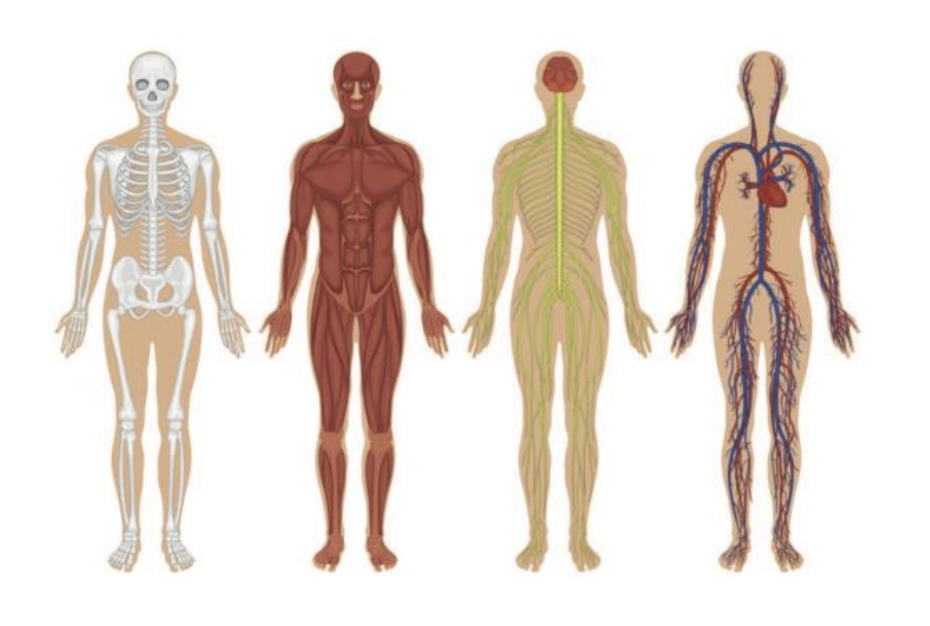
\includegraphics[scale=0.5]{figs/Q4}
\end{figure}
\end{enumerate}


\پاسخ{

\begin{enumerate}[a)]
		\item 
معماری نرم‌افزار بخش مهمی از قسمت طراحی (\lr{design}) در چرخه‌ی عمر توسعه نرم‌افزار است. معماری مانند یک نقشه‌ی کلی برای سیستم عمل می‌کند و انتزاعی بودن باعث مدیریت پیچیدگی سیستم و ایجاد هماهنگی بین اجزا می‌شود. به علاوه در طراحی نرم‌افزار، عناصر یک سیستم، نحوه تناسب آنها و چگونگی همکاری با یکدیگر برای برآوردن نیازهای سیستم توصیف می‌شود. از این لحاظ می‌توان بیان کرد که معماری نرم‌افزار بخش مهمی در طراحی نرم‌افزار است. البته می‌توان نوع ارتباط دیگری هم در پیش‌زمینه مدنظر داشت: یکی از مهمترین اهداف معماری نرم‌افزار مشخص کردن نیازمندی‌هایی است که ساختار نرم‌افزار را تحت تاثیر قرار می‌دهد و به این صورت خطرات تجاری که هنگام بررسی مسائل فنی به وجود می‌آیند را خنثی می‌کند. از این لحاظ می‌توان گفت معماری به بخش تحلیل نیازمندی‌ها (\lr{Requirement analysis}) هم مرتبط است.
		
		\item 
		\begin{enumerate}
	\item قابلیت نگه‌داری کد بهتر \\
با داشتن یک معماری خوب نگه‌داری از کد بهتر و راحت‌تر صورت می‌گیرد زیرا ساختار کد شفاف و شناخته‌شده است بنابراین راحت‌تر می‌توان به دنبال مشکلات و باگ‌ها گشت.

	\item تطبیق‌پذیری بهتر \\
ساخت ویژگی‌های فنی جدید یا یک مساله تجاری جدید ساده‌تر قابل دسترسی خواهد بود زیرا معماری خوب یک سیستم باعث شفافیت و بخش‌بندی قسمت‌های مختلف می‌شود.
	\item ساخت مدلی با قابلیت استفاده مجدد \\
معماری تثبیت‌شده ممکن است دوباره برای محصولات دیگراستفاده شود، مخصوصا اگر محصولات دارای نیازمندی‌های مشابه باشند. وقتی کدی مجددا استفاده می شود، در مصرف منابعی مانند زمان و پول صرفه‌جویی می‌شود. مهمتر از آن، کیفیت نرم افزاری که reuse شده، افزایش می یابد زیرا این کد قبلاً تست شده است.
	\item کاهش تکرار و هزینه‌های ناشی از آن \\
یک معماری درست باعث شفافیت می‌شود و به صورت کلی نقاط مختلف و وابستگی بینشان را مشخص می‌کند. بنابراین کمک می‌کند تا دوگانگی (duplicity) کمتری در کد داشته باشیم و هزینه‌های رسیدگی به این دوگانگی‌ها را در آینده کاهش می‌دهد.
	\item مشخص کردن راه‌حل برای نیازمندی‌ها \\
س از دریافت نیازمندی‌ها از Stakeholderها،  یک نرم‌افزار سعی می‌کند تمامی نیازمندی‌های کاربردی، غیر کاربردی و … را پوشش دهد. در این صورت یک معماری درست راه‌حلی برای ارضای نیازمندی‌‌های مختلف ارائه می‌دهد زیرا یک معماری درست پایه و اساس نرم‌افزار است و نرم‌افزارهایی که فاقد یک معماری مستحکم هستند به خوبی نمی‌توانند همه‌ی نیازمندی‌ها را برآورده کنند.

\end{enumerate}
		
	
		\item
در تصویر زیر قسمت‌های مختلف بدن انسان و اتصالات درونی هر قسمت نشان داده شده است. مثلا ساختار استخوان‌بندی، عصب‌بندی و ارتباط آن با مغز، ساختار رگ و عروق و ارتباط آن با قلب و همچنین ساختار توزیع ماهیچه‌ها در بدن. همه‌ی این قسمت‌ها در تصویر زیر مشخص شده‌اند و در واقع یک نقشه‌ی کلی برای ساخت یک انسان داریم! و در صورتی که مشکلی برای قسمتی از بدن پیش بیاید می‌توان با این نقشه‌ها مشخص کرد مشکل از کدام ساختار از بدن است؛ آیا مشکل عصبی وجود دارد یا استخوانی به مشکل خورده؟ همچنین باید ارتباط بین این بخش‌ها مشخص شود و به این صورت یک معماری کامل از بدن انسان خواهیم داشت. پس در کل می‌توان گفت معماری یک نرم‌افزار هم مانند یک تصویر نقشه‌ای از قسمت‌های مختلف، نحوه‌ی توزیع این قسمت‌ها و ارتباط بین بخش‌های مختلف را نمایش می‌دهد.
	\end{enumerate}

\subsection*{مراجع}

\begin{latin}
	\begingroup
	\renewcommand{\section}[2]{}%
	
	\begin{thebibliography}{9}
	
\bibitem{phoenixnap}
PhoenixNAP,
\textit{Seamless development: focus on the essential}.
Accessed on 1/11/2023,
\url{https://www.eiffel.com/values/seamless-development/}

\bibitem{tp}
tutorialspoint,
\textit{Software Architecture \& Design Introduction}.
Accessed on 1/11/2023,
\url{https://www.tutorialspoint.com/software_architecture_design/introduction.htm}

\bibitem{wp}
wikipedia,
\textit{Software architecture - Wikipedia}.
Accessed on 1/11/2023,
\url{https://en.wikipedia.org/wiki/Software_architecture}

\bibitem{apiumhub}
Apiumhub,
\textit{15 benefits of software architecture you should know}.
Accessed on 1/11/2023,
\url{https://apiumhub.com/tech-blog-barcelona/benefits-of-software-architecture/#15_benefits_of_software_architecture}

\bibitem{linkedin}
Linkedin,
\textit{8 Reasons why software architecture is important?}.
Accessed on 1/11/2023,
\url{https://www.linkedin.com/pulse/8-reasons-why-software-architecture-important-ahad-khan-csm/}
		
	\end{thebibliography}
	\endgroup
\end{latin}

}
